\chapter{Physics Objects}

\todo[inline]{introduction to reconstruction of physics objects.}

\begin{figure}[htb]
  \centering
  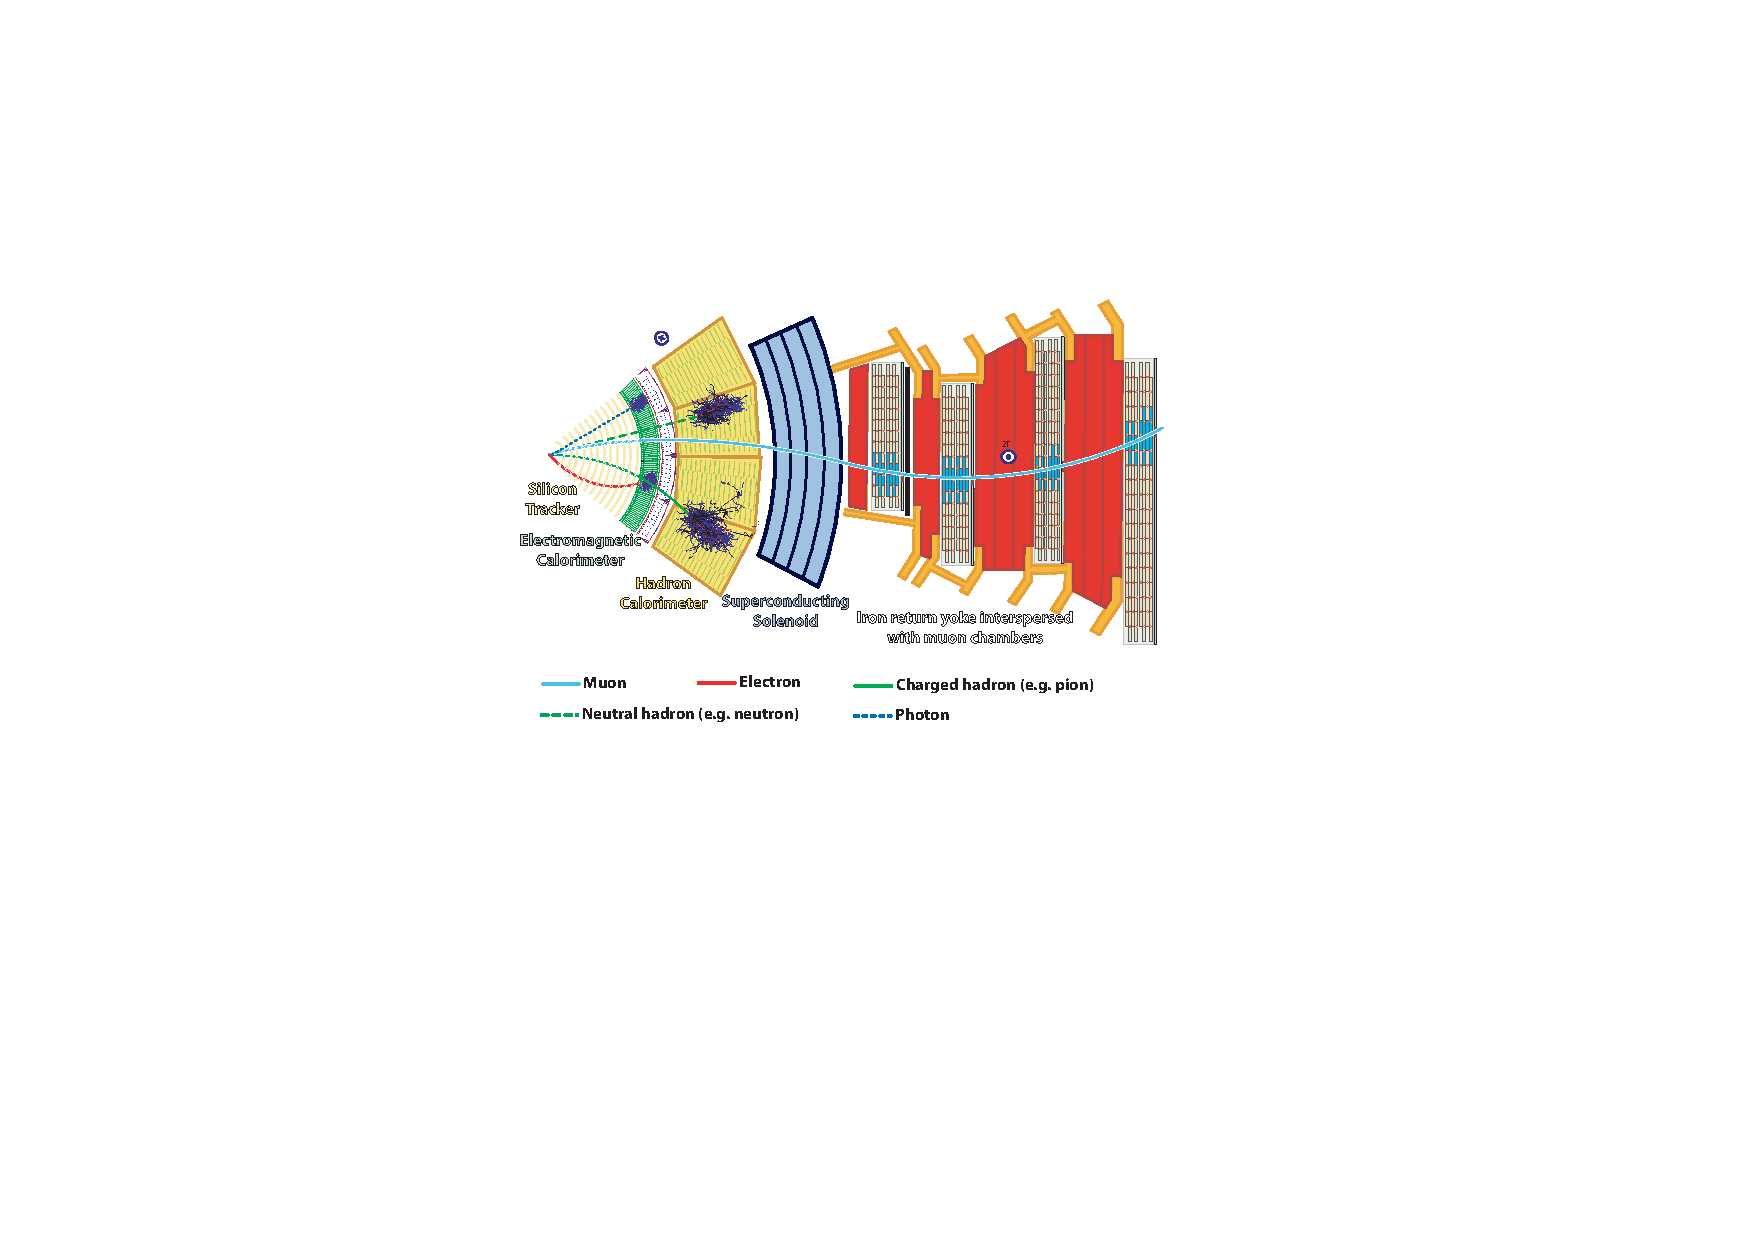
\includegraphics[width=0.5\textwidth]{slice}
  \caption{The path of different particles through a cross section of the CMS detector.}
  \label{reco:crosssec}
\end{figure}

\section{Electrons}
\todo[inline]{Why are electrons important phsyics objects}
\todo[inline]{Describe path that electrons make through the detector.}

\subsection{Triggering}

\subsection{Reconstruction}
Electrons are reconstructed in CMS using information from the pixel detector,
silicon strip tracker and the ECAL.

\subsubsection{Electron Clustering}
As electrons traverse the CMS tracker, the strong magnetic field causes the path
of the electrons to be curved in the azimuthal, $\phi$, direction. The electrons
radiate bremsstrahlung photons, so that when the electron energy reaches the
ECAL it is spread over a narrow strip in the phi direction.
\FigureRef{reco:brem} shows the fraction of energy radiated by bremsstrahlung for
electrons of energy $10$, $30$ and \unit{$50$}{\GeV}.

\begin{figure}[htb]
  \centering
  %
\includegraphics[width=0.5\textwidth]{placeholder}
  \missingfigure{Fraction of energy radiated by bremsstrahlung from Electron
reconstruction in CMS}
  \caption{Fraction of electron energy, $E^{e}$, radiated away as bremsstrahlung
photons, $\sum E_{brem}^{\gamma}$ for electrons of energy }%$10$, $30$ and \unit{$50$}{\GeV}. From \cite{}.}
  \label{reco:brem}
\end{figure}

To measure the electron energy, including the bremsstrahlung photons, the
seperated deposits of energy need to be collected, using super-clustering
algorithms. 

In the barrel a ``hybrid'' algorithm is used. The hybrid algorithm proceeds by
identifying several hot crystals, with energies above a certain threshold, that
will act as seeds. The algorithm then forms $1\times3$ or $1\times5$ crystal
``dominos'', centered on the seed crystal, depending on the energy within the
domino. The dominos are then collected together in the $\phi$ direction, up to
an extension of \unit{0.3}{\rad}, to form clusters of clusters. This is
demonstrated in \FigureRef{fig:hybrid}.

\begin{figure}[htb]
  \centering
  %
\includegraphics[width=0.5\textwidth]{placeholder}
  \missingfigure{hybrid clustering algorithm}
  \caption{Demonstration of the clustering of dominos in the hybrid algorithm.}
  \label{reco:hybrid}
\end{figure}

A ``multi5x5'' algorithm is used in the ECAL endcaps. Energy is collected in
$5\times5$ matrices, which are then collected together if their position lies on
a narrow $\phi$ road to form superclusters.

\subsubsection{Electron Seeding}
The superclusters are then used to select seeds for the track reconstruction.
Starting with a supercluster that passes a \pt and a hadronic veto, the
trajectory of the electron is propogated back through the magnetic field and
matched to the trajectory seeds, pairs or triplets of hits in the inner tracker.
If the trajectory seeds fall within a window of the supercluster path under
either charge hypothesis, they are selected and used to seed the track
reconstruction.
The ECAL driven seeding is comlemented by a tracker driven seeding algorithm.
This starts with high purity tracks and extrapolating them outwards to the ECAL.
This is effective for lower \pt electrons.

Seeds from both of the algorithms are collected and merged in to a single
collection, which is then used to seed the electron track reconstruction.

\subsubsection{Electron Track Reconstruction}
\todo[inline]{Rewrite this section}
The track reconstruction is based on a combinatorial Kalman filter,\todo{find a
citation for this} with the electron energy losses described using Bethe Heitler
modelling.

The track reconstruction starts with a seed, from which a tree of possible track
candidates is built from. 

%track reconstruction paper
Throughout the track reconstruction, tracks candidates are described by a state
vector containing information on the momentum, direction and position of the
track.

The Kalman filter is a
two step process. In the propogation step, track states are extrapolated to
the next layer of the detector, while taking in to account for energy losses due
to bremsstrahlung and coulomb scattering. 
In the update step, the extrapolated track state is 
combined with what is observed in that layer and the track is updated. 

The collected hits are passed to the GSF for a final fitting and estimation of
the track parameters. The GSF algorithm is similar to the Kalman filter but
energy losses are now described by a weighted sum of Gaussian distributions.
% corrections

\subsection{Electron Identification}
Electron identifiaction is based on a limited number of variables.
\todo{backgrounds to prompt electrons}

\subsubsection{Shape variable }

$\sigma_{\eta\eta}$ is the width of the electron shower in the $\eta direction$,
\begin{equation}
\sigma_{\eta\eta} = 
\sum_{\text{crystals}} \left(\eta_{i} - \eta{s}\right)^{2}
\frac{E_{i}}{E_{\text{seed cluster}}}.
\end{equation}

\subsubsection{Hadronic Energy}
Ratio of the energy deposited in the HCAL tower behind the electromagnetic seed
cluster to the energy of that seed cluster.

\subsubsection{Angular Separation of Track and Super Cluster}
$\Delta\phi$ and $\Delta\eta$ represent the angular separation between the
trajectory of the reconstucted GSF track, extrapolated to the ECAL, and the ECAL supercluster in the $\phi$
and $\eta$ direction respectivly.
\begin{align}
|\Delta\eta| &\equiv |\eta_{\text{SC}} - \eta_{track}|\\
|\Delta\phi| &\equiv |\phi_{\text{SC}} - \phi_{track}|
\end{align}

\subsubsection{Isolation}
For the calorimeter quantities

\subsubsection{Conversion Rejection}
Three further variables are included to reject electrons that are produced from
photon conversions. The missing hits is simply the number of layers in the inner
tracker where an expected hit from the track reconstruction is not detected by
the detector.
\todo{coversion partner tracks and dist and cot}
Coversion partner tracks are track candidates that are with in a cone of $\Delta
R < 0.3$ around the electron candidate track, and have an opposite charge. The
following two variables are used to detect \todo{what?} conversions.

\begin{equation}
\Delta \cot \theta \equiv \cot(\theta_{\text{KF}}) - \cot(\theta_{\text{GSF}})
\end{equation}
where $\theta_{KF}$ and $\theta_{GSF}$ are the polar angle of the conversion
partner track and the GSF track of the electron respectivly.

The variable, dist, is the distance between the two tracks where they are
parralel. \FigureRef{fig:dist} describes dist.

\begin{figure}[htb]
  \centering
  \missingfigure{Explanation of dist}
  %
\includegraphics[width=0.5\textwidth]{placeholder}
  \caption{Dist is the distance between}
  \label{fig:dist}
\end{figure}

\subsubsection{Electron Identification Working Points}

Several sets of cuts have been produced for CMS analyses with different
efficiencies in mind. The cut values are sumarised in \TableRef{tab:electronwp}.
\todo{table of electron working points}

\subsection{Charge Identification}
The charge of an electron can be identified by studying how the electron trajectory
is bent in the magnetic field as the electron passes through the tracker. This
can be made difficult by conversion of bremsstrahlung photons when they are
radiated early. 

Within CMS, three methods of charge identifaction have been developed based on
the GSF track charge, the general track charge and the supercluster charge. The
GSF track charge is simply the sign of the curvature of the GSF fit of the
electron track. The general track charge is found by matching the GSF track with
general Kalman filter track by asking for shared hits in the pixel tracker. 
The super cluster charge is obtained by finding the sign of the phi difference
between the supercluster position and the first hit of the electron track.

At the \PZ peak, a charge mis-identification rate of \unit{3}{\%} is expected,
when using the electron trajectory from the GSF fit.  A sample with improved
charge identifaction can be obtained by using a majority method, that combines
the three measurements and assigns the sign from the 2 estimates out of three
that are in agreemenet, or by requiring that all three methods for assigning
charge are in agreement and discarding the event otherwise.

\section{Missing Energy}
\todo[inline]{Describe how MET is measured in CMS} 

\subsection{Particle Flow at CMS}
\todo[inline]{Tie particle flow in with rest of chapter.} 

New physics will manifest itself in CMS through signatures involving standard
model particles. Important signatures for many new phenomena include high \Pt\
jets, missing transverse energy (\met), jets containing \Pbottom quarks and
hadronically decaying tau leptons. To study these signatures it is important to
reconstruct and identify all particles in events as accurately as possible. The
particle-flow event reconstruction attempts to reconstruct and identify all
stable particles in an event by combining information from all CMS
sub-detectors. The particle reconstruction and identification starts with
collecting information from each subdetector to form elements such as tracks
and energy clusters in the calorimeters. These basic 'elements' are then
combined to form blocks which are then interpreted in terms of particles by the
particle flow algorithm. A list of individual particles is then returned from
the algorithm which can be used to study the event in greater detail by,
amongst other things, building jets, tagging b quarks and calculating missing
transverse energy.\cite{PF}

The first step of the particle-flow reconstruction algorithm is to collect the
fundamental elements. The elements consist of charged particles tracks from the
tracker, clusters of energy deposition in the calorimeters and muon tracks.
These elements need to be identified with a high efficiency and low fake rate
since the particle reconstruction depends on these basic elements and
misidentified elements could lead to missing or double counted
particles.\cite{PF}

As a particle traverses the detector it may interact with many CMS subdetectors
creating several particle-flow elements. A link algorithm is used to connect
the elements together to form blocks that typically contain 1, 2 or 3 elements.
The algorithm returns a distance between the elements as a measure of the
quality of the link. The final step of the particle flow algorithm is to
reconstruct and identify particles from each block of linked elements.\cite{PF}

Once the event has been fully reconstructed with the particle flow technique
the missing transverse energy (\met) in the event can be easily computed by
summing up the transverse momentum of all the reconstructed particles.\cite{PF}

